\documentclass{article}

\usepackage[francais]{babel}
\usepackage[T1]{fontenc}
\usepackage{moreverb}       % verbatim with tab

\usepackage{wrapfig}
\usepackage{graphicx}
\usepackage{geometry}
\geometry{hmargin=2.5cm}
\usepackage{amsmath}
\usepackage{siunitx}

\usepackage{graphicx}
\usepackage{subcaption}
\usepackage{float}
\usepackage{hyperref}
\usepackage{setspace}
\usepackage{xcolor}
\usepackage{pdfpages}
\usepackage{enumitem}
\usepackage{lscape}

\usepackage{fancyhdr}       % en-têtes
\usepackage{lastpage}       % numéro de dernière page

\title{Réseaux industriels}
\date{2020}
\author{Laura Bin}

\pagestyle{fancy}
\renewcommand\headrulewidth{1pt}
\fancyhead[L]{Laura Binacchi}
\fancyhead[C]{Réseaux industriels}
\fancyhead[R]{\today}

\begin{document}
    \pagenumbering{arabic}

    \begin{center}
        \textbf{\LARGE Travail sur les librairies}
    \end{center}

    \paragraph{}
    A l’aide de la librairie réalisée dans l’exercice précédent, réaliser une application client-serveur s’échangeant une liste d’éléments. Le client générera la liste contenant un nombre d’éléments passés en argument. Chaque élément contiendra un entier, une chaîne de caractère et un flottant qui seront différents pour chaque élément de la liste (ces données pourront être générées aléatoirement ou suivre une règle que vous inventerez). Le client enverra la liste au serveur et celui-ci affichera la liste à l’écran. L’envoi des données se fera en suivant le point \href{https://beej.us/guide/bgnet/html/#serialization}{7.4. Serialization—How to Pack Data} de la documentation.


    \section{Définition de la structure de données}
    \paragraph{}
    Le structure de données envoyée du client au serveur une liste chaînée qui rassemble différents types de données\footnote{Cette structure est définie dans le fichier \emph{data.h}.} :
    \begin{verbatimtab}
        struct data_node {
            int16_t int_16;             // 16 bytes integer
            int32_t int_32;             // 32 bytes integer
            int64_t int_64;             // 64 bytes integer
            float   f;                  // 32 bytes float
            double  d;                  // 64 bytes double
            char    *str;               // string
            struct data_node *next;     // next node
            };
    \end{verbatimtab}

    \paragraph{}
    Elles peuvent être affichées sous la forme suivante par la méthode \texttt{print\_list} qui permet d'afficher l'intégralité d'une liste chaînée\footnote{Comme pour toutes les méthodes concernant la structure de données, le prototype de cette méthode est défini dans le fichier \emph{data.h} et son implémentation est réalisée dans le fichier \emph{data.c}.} :
    \begin{verbatimtab}
        Node x/TOTAL {
            int_16: 18132
            int_32: 1217769723
            int_64: 9223372036120782570
            float:  54783.093750
            double: -316265447.685803
            string: e04tiD51hvLxeai
        }
    \end{verbatimtab}

    \newpage
    \paragraph{}
    Ces données sont générées aléatoirement par la méthode \texttt{create\_node}.
    
    \paragraph{}
    La liste peut ensuite être envoyée par le client avec \texttt{send\_list} et reçue par le serveur avec \texttt{receive\_list}. L'envoi commence par l'envoi d'un packet contenant le nombre de structures de données (nodes) qui vont être envoyées. Puis chaque structure est envoyée dans un packet indépendant précédé de sa taille. Ces headers permettent au seveur d'attendre d'avoir reçu un node entier (au cas où les packets seraient envoyés en plusieurs fois par la couche réseau) avant de le désérialiser pour composer sa propre liste de données.

    \paragraph{}
    Enfin, le serveur envoie un acknowledgement contenant la somme de bytes reçue (0 en cas d'erreur lors de la réception) avec \texttt{send\_ack} et le client le reçoit avec \texttt{receive\_ack}.

    \paragraph{}
    Cette liste de données peut être composée de 1 à 65535 nodes. Il n'est donc pas possible d'envoyer une liste vide.


    \section{Réalisation de la librairie}
    \paragraph{}
    Pour que le client puisse envoyer les données et que le serveur puisse les recevoir, les méthodes d'envoi et de réception vont faire appel à une librairie de sérialisation. Les prototypes des fonctions de cette librairie \emph{libserial} sont définis dans \emph{serial-util.h} et leur implémentation est réalisée dans \emph{serial-util.c}.

    \paragraph{}
    Fonctions d'écriture d'une donnée dans un buffer :
    \begin{itemize}
        \item \texttt{char *write\_u16(uint16\_t i, char *out\_buf)} : writes a given 16 bytes unsigned integer in the buffer
        \item \texttt{char *write\_u32(uint32\_t i, char *out\_buf)} : writes a given 32 bytes unsigned integer in the buffer
        \item \texttt{char *write\_u64(uint64\_t i, char *out\_buf)} : writes a given 64 bytes unsigned integer in the buffer
        \item \texttt{char *write\_f32(float f, char *out\_buf)} : writes a given 32 bytes float in the buffer
        \item \texttt{char *write\_f64(double d, char *out\_buf)} : writes a given 64 bytes double in the buffer
        \item \texttt{char *write\_str(char *str, char *out\_buf)} : writes a given string in the buffer
    \end{itemize}

    \paragraph{}
    Fonctions de lecture d'un buffer vers une donnée :
    \begin{itemize}
        \item \texttt{char *read\_u16(char *buf, uint16\_t out\_i)} : reads a 16 bytes unsigned integer from the buffer
        \item \texttt{char *read\_u32(char *buf, uint32\_t out\_i)} : reads a 32 bytes unsigned integer from the buffer
        \item \texttt{char *read\_u64(char *buf, uint64\_t out\_i)} : reads a 64 bytes unsigned integer from the buffer
        \item \texttt{char *read\_f32(char *buf, float out\_f)} : reads a 32 bytes float from the buffer
        \item \texttt{char *read\_f64(char *buf, double out\_d)} : reads a 64 bytes double from the buffer
        \item \texttt{char *read\_str(char *buf, char *out\_str)} : reads a string from the buffer
    \end{itemize}

    \paragraph{}
    La sérialisation est faite en big-endian. Pour sérialiser les float et double, j'extraistre l'exposant et la mantisse (qui conserve son signe) que je sérialise sous forme d'entiers de taille fixe.

    \section{Structure du projet}
    \paragraph{}
    Puisque la librairie TCP est maintenant partagée entre le projet précédent et ce projet, les librairies sont maintenant placées dans un répertoire qui se trouve au même niveau que ceux des projets :
    \begin{verbatimtab}
        - ex-lib
            + include
            + src
            Makefile
        - ex-serial
            + include
            + src
            Makefile
        - include
            serial-util.h
            tcp-util.h
        - lib
            serial-util.c
            tcp-util.c
        Makefile
    \end{verbatimtab}


    \section{Compilation du projet}
    \paragraph{}
    Puisque la structure des dossiers a été modifiée, le \emph{Makefile} du projet précédent doit être légèrement modifié. L'arborescence de fichiers présentée au point précédent montre qu'il y a maintenant un \emph{Makefile} principal à la racine des projets qui peut appeler les \emph{Makefile} des sous-projets (ensemble ou séparément).

    \paragraph{}
    Le \emph{Makefile} principal compile d'abord les librairies avec les mêmes commandes que pour le projet précédent :
    \begin{verbatimtab}
[1]         cc -g  -Wall -Wpedantic -Wextra -Iinclude -Wl,-soname,libtcp.so.1
                -shared -fPIC -o lib/libtcp.so.1.0 lib/tcp-util.c
[2]         ldconfig -r lib -n .
[3]         ln -sf libtcp.so.1 lib/libtcp.so
[4]         cc -g  -Wall -Wpedantic -Wextra -Iinclude -Wl,-soname,libserial.so.1
                -shared -fPIC -o lib/libserial.so.1.0 lib/serial-util.c
[5]         ldconfig -r lib -n .
[6]         ln -sf libserial.so.1 lib/libserial.so
    \end{verbatimtab}

    \begin{description}
        \item[\texttt{[1]} ] La librairie \emph{libtcp} est compilée dans sa version 1.0 (fichier de sortie : \emph{lib/libtcp.so.1.0}) à partir du fichier \emph{lib/tcp-util.c}. Elle sera référencée via sa version majeure (\emph{libtcp.so.1}) par les projets qui en dépendent. Le compilateur utilisé est cc, en mode debug et avec warnings supplémentaires.
        \item[\texttt{[2]} ] Création d'un lien symbolique de la version 1 de ma librairie (\emph{libtcp.so.1}) vers la version 1.0 (\emph{libtcp.so.1.0})
        \item[\texttt{[3]} ] Création d'un lien symbolique de la librairie (\emph{libtcp.so}) vers la version 1 (\emph{libtcp.so.1})
        \item[\texttt{[4-6]} ] Les mêmes opérations sont répétées pout la librairie \emph{libserial}
    \end{description}

    \paragraph{}
    Le \emph{Makefile} compile ensuite le projet \emph{ex-serial} :
    \begin{verbatimtab}
[1]         gmake -C ex-serial
[2]         gmake[1]: Entering directory '/home/lbin/Documents/2020_RI/ex-serial'
[3]         mkdir out
[4]         cc -g  -Wall -Wpedantic -Wextra -Iinclude -I../include
                -c -o out/data.o src/data.c
[5]         cc -g  -Wall -Wpedantic -Wextra -Iinclude -I../include 
                -Wl,-rpath='\$ORIGIN/../lib' -o client src/client.c
                out/data.o ../lib/libtcp.so ../lib/libserial.so
[6]         cc -g  -Wall -Wpedantic -Wextra -Iinclude -I../include
                -Wl,-rpath='\$ORIGIN/../lib' -o server src/server.c
                out/data.o ../lib/libtcp.so ../lib/libserial.so
[7]         gmake[1]: Leaving directory '/home/lbin/Documents/2020_RI/ex-serial'
    \end{verbatimtab}

    \begin{description}
        \item[\texttt{[1]} ] Exécution du \emph{Makefile} du projet \emph{ex-serial} par le \emph{Makefile} principal
        \item[\texttt{[2]} ] \emph{gmake} se déplace dans le répertoire du projet
        \item[\texttt{[3]} ] Création du répertoire \emph{out} si il n'existe pas
        \item[\texttt{[4]} ] Compilation du fichier \emph{data.c} en fichier objet \emph{data.o}
        \item[\texttt{[5]} ] Compilation du fichier \emph{client.c} en fichier exécutable \emph{client} avec les dépendances aux librairies \emph{libtcp} et \emph{libserial} (ces librairies se trouvent dans le répertoire \emph{lib} du répertoire parent)
        \item[\texttt{[6]} ] Même opération que \textbf{\texttt{[5]}} pour le \emph{server}
        \item[\texttt{[7]} ] \emph{gmake} retourne dans le répertoire parent
    \end{description}

    
    \section{Installation du client et du serveur}
    \paragraph{}
    Je commence par compiler le projet \emph{ex-serial} en local en exécutant la commande \texttt{gmake ex-serial} dans le répertoire à la racine de mes projets :
    \begin{figure}[H]
        \centering
        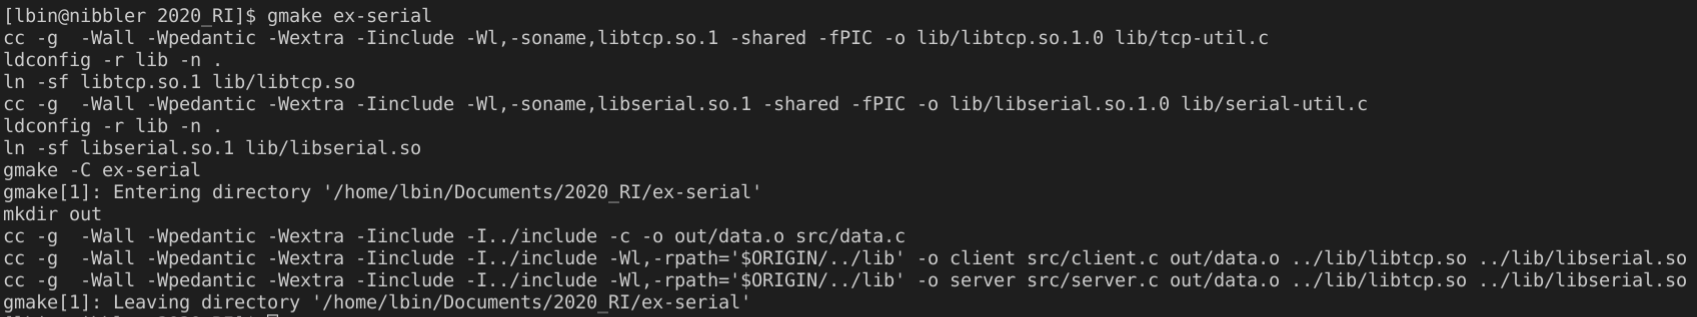
\includegraphics[width=\linewidth]{./screenshots/compilation.png}
    \end{figure}

    \newpage
    \paragraph{}
    Je copie ensuite les exécutales sur mes machines virtuelles et puisque la structure de mes répertoires a changé, je remonte de dossier \emph{lib} dans le répertoire racine de mes projet :
    \begin{figure}[H]
        \centering
        \begin{subfigure}[b]{.48\textwidth}
            \centering
            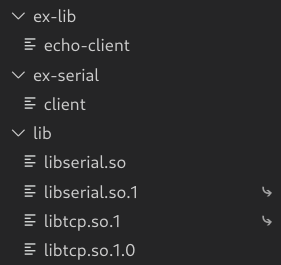
\includegraphics[width=.5\textwidth]{./screenshots/client-arbor.png}
        \end{subfigure}
        \begin{subfigure}[b]{.48\textwidth}
            \centering
            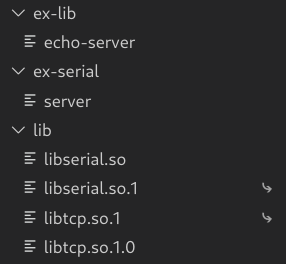
\includegraphics[width=.5\textwidth]{./screenshots/server-arbor.png}
        \end{subfigure}
    \end{figure}

    \paragraph{}
    Comme pour le projet précédent, les liens symboliques ont été recréés avec la commande \texttt{ldconfig -n .} :
    \begin{figure}[H]
        \centering
        \begin{subfigure}[b]{.48\textwidth}
            \centering
            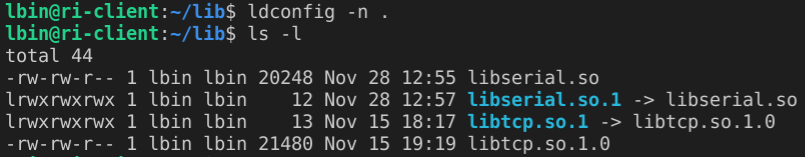
\includegraphics[width=\textwidth]{./screenshots/client-liens-symb.png}
        \end{subfigure}
        \begin{subfigure}[b]{.48\textwidth}
            \centering
            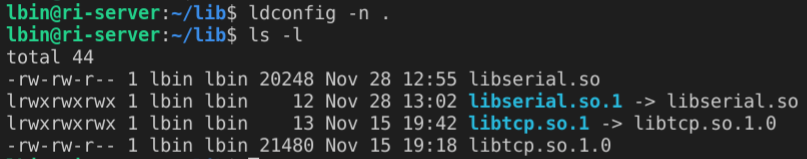
\includegraphics[width=\textwidth]{./screenshots/server-liens-symb.png}
        \end{subfigure}
    \end{figure}

    \paragraph{}
    Et les fichiers \emph{client} et \emph{server} ont été rendus exécutables :
    \begin{figure}[H]
        \centering
        \begin{subfigure}[b]{.48\textwidth}
            \centering
            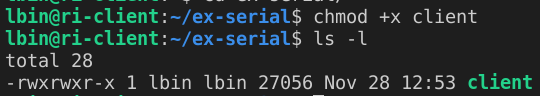
\includegraphics[width=.8\textwidth]{./screenshots/client-exec.png}
        \end{subfigure}
        \begin{subfigure}[b]{.48\textwidth}
            \centering
            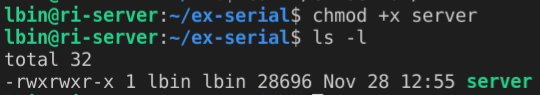
\includegraphics[width=.8\textwidth]{./screenshots/server-exec.png}
        \end{subfigure}
    \end{figure}


    \newpage
    \section{Tests}
    \subsection{Envoi d'une liste courte}
    \paragraph{}
    Après avoir démarré le serveur (sans \texttt{sudo} puisque je n'utilise plus le port réservé au protocole echo), je lui envoie une liste de trois éléments via le client :
    \begin{figure}[H]
        \centering
        \begin{subfigure}[b]{.48\textwidth}
            \centering
            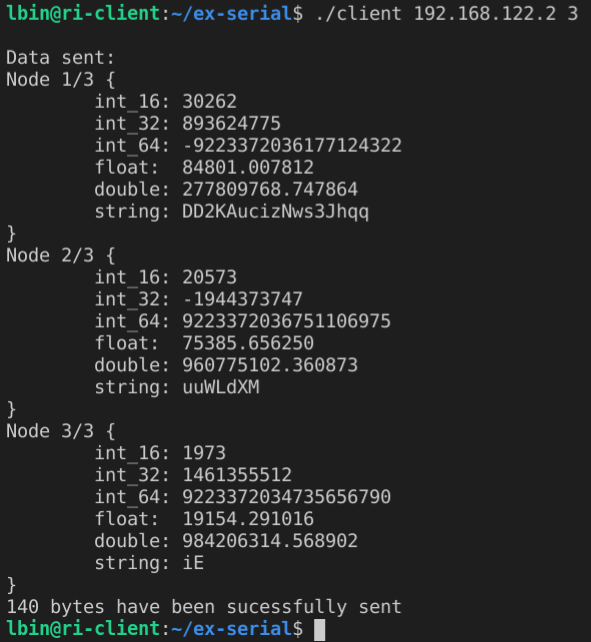
\includegraphics[width=\textwidth]{./screenshots/client-test-simple.png}
        \end{subfigure}
        \begin{subfigure}[b]{.48\textwidth}
            \centering
            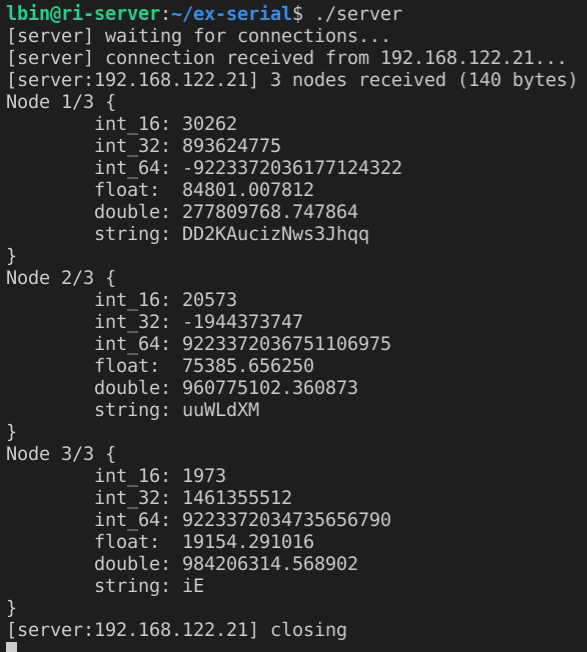
\includegraphics[width=.98\textwidth]{./screenshots/server-test-simple.png}
        \end{subfigure}
    \end{figure}

    \paragraph{}
    Le serveur a bien reçu les 140 bytes envoyés par le client. Les données reçues et affichées correspondent bien à celles envoyées par le client. Le serveur ferme la connection avec le client et est prêt à en recevoir une nouvelle.

    \subsection{Envoi d'une liste vide}
    \paragraph{}
    L'envoi d'une liste vide n'est simplement pas rendu possible par le programme du client :
    \begin{figure}[H]
        \centering
        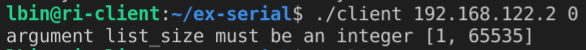
\includegraphics[width=.45\linewidth]{./screenshots/client-test-0.png}
    \end{figure}

    \paragraph{}
    Il en va de même pour les listes contenat un nombre d'éléments allant au-delà de 65535, un nombre négatif d'éléments, ou lorsqu'une chaîne de caractères est entrée à la place du nombre :
    \begin{figure}[H]
        \centering
        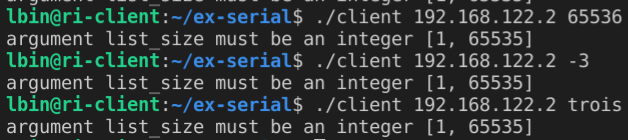
\includegraphics[width=.45\linewidth]{./screenshots/client-test-valeurs-hors-limite.png}
    \end{figure}

    \subsection{Envoi d'une liste de 65535 éléments}
    \paragraph{}
    Par contre, l'envoi fonctionne bien avec une liste de 65535 éléments\footnote{Pour plus de facilité de lecture, pour ce test, j'ai modifié la fonction d'impression pour qu'elle n'affiche que les trois premiers éléments de la liste.} :
    \begin{figure}[H]
        \centering
        \begin{subfigure}[b]{.48\textwidth}
            \centering
            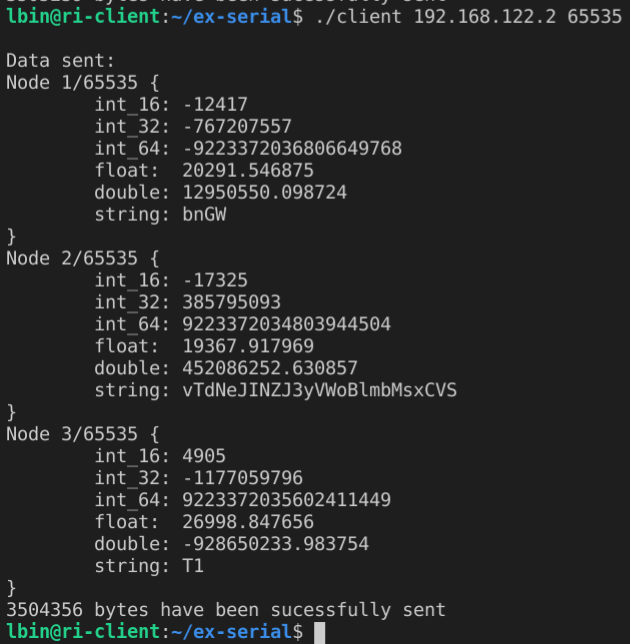
\includegraphics[width=.96\textwidth]{./screenshots/client-test-65535.png}
        \end{subfigure}
        \begin{subfigure}[b]{.48\textwidth}
            \centering
            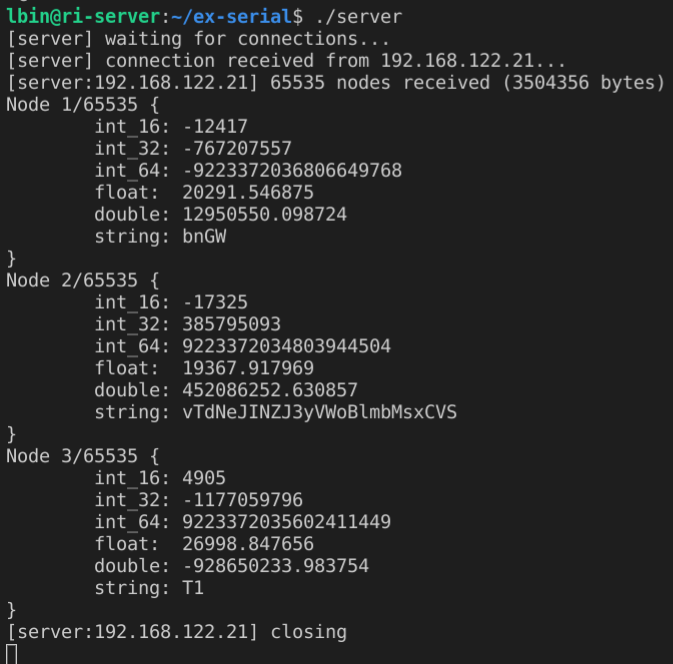
\includegraphics[width=\textwidth]{./screenshots/server-test-65535.png}
        \end{subfigure}
    \end{figure}
\end{document}
